\documentclass{article}
\usepackage[pdftex]{graphicx}
\usepackage[export]{adjustbox}
\usepackage{amsmath}
\usepackage{amssymb}
\usepackage[dutch]{babel}
\usepackage{fullpage}
\usepackage{epsfig}
\usepackage[T1]{fontenc}
\usepackage{epstopdf}
\usepackage{relsize}
\newcommand{\zv}{\blacksquare}
\newcommand{\wv}{\square}
\newcommand{\R}{\mathbb{R}}
\newcommand{\N}{\mathbb{N}}
\usepackage{float}
\usepackage[caption = false]{subfig}
\usepackage{graphicx}
\usepackage{tikz}
\usetikzlibrary{matrix}

\begin{document}

\title{Elliptische Kromme Diffie-Hellman}

\author{R.L. Neuteboom (4006712) S.E.M.P. Franssen(4035844)\\
\small Universiteit Utrecht \normalsize}

\date{3 Juli 2015}
\maketitle
\section{Inleiding}
Tegenwoordig is het steeds belangrijker om communicatie, die via het internet wordt verspreid, te versleutelen. Zelfs als informatie nietszeggend lijkt te zijn, kunnen mensen, die de gegevens onderscheppen, daar veel uit opmaken. Een voorbeeld hiervan heb ik gezien bij een gastcollege van het vak Databases. De gastspreker liet zien dat je, met geringe informatie over \'e\'en persoon, vaak relatief eenvoudig uit een grote database een kleine groep kan aanwijzen waar die persoon zich in bevindt. Dit kan bijvoorbeeld door een variant van binary search te gebruiken. Om een groep van $n$ personen te onderscheiden, heb je $O(log(n))$ ja/nee vragen nodig. Dit heeft als gevolg dat je ongeveer $33$ goede ja/nee vragen nodig hebt om elk persoon op aarde uniek te identificeren.
Volgens artikel 138a van het Wetboek van Strafrecht (computervredebreuk) is het verboden om toegang te verwerven door het doorbreken van beveiliging, dan wel een technische ingreep, of met behulp van valse signalen of een valse sleutel, of door het aannemen van een valse hoedanigheid. Omdat je met bijvoorbeeld wireshark alle paketten die jouw pc ontvangt inzichtelijk kan maken, kun je hiermee verkeer afluisteren. Dit valt buiten de wet op computervredebreuk, omdat je alleen inzichtelijk maakt welke berichten jouw pc heeft ontvangen. De berichten zijn al door jouw pc ontvangen.\\
In dit verslag wordt beschreven hoe je het Diffie-Hellman protocol kunt gebruiken om versleutelde communicatie op te zetten. Voor dit protocol is een systeem nodig om in te werken. Het systeem dat we gebruiken zal bestaan uit een eindige cyclische multiplicatieve groep. We cre\"eren deze met behulp van een elliptische kromme. Verder willen we het bericht ondertekenen, dit zodat de ontvanger weet dat het van ons komt. Het kan namelijk zo zijn dat iemand anders contact probeert te zoeken met de ontvanger en valse berichten stuurt. Ten slotte gaan we in op hoe we deze technieken/algoritmen hebben ge\"implementeerd in Python.
\newpage
\section{Diffie-Hellman protocol}
Het Diffie-Hellman protocol is een manier om een sleutel af te spreken die vervolgens gebruikt kan worden voor versleutelde communicatie. De effectiviteit van het protocol is gebaseerd op het feit dat een bepaalde bewerking niet makkelijk om te keren is, bijvoorbeeld multiplicatie in een bepaalde groep.\\
De bedoeling is dat een bericht van A naar B gestuurd kan worden, zonder dat anderen, E, die het bericht onderscheppen, het kunnen begrijpen. Dit is het principe van Cyptografie. Binnen de Cryptografie is het standaard  dat A met Alice, B met Bob en de afluisteraar met Eve wordt aangeduid. Als ergens in de tekst het woord \emph{openbaar} wordt gebruikt, betekent dat ook derden die informatie kunnen ontvangen en lezen.  
Het Diffie-Hellman protocol gaat als volgt te werk:
\begin{itemize}
\item Alice en Bob communiceren in het openbaar het systeem dat ze gaan gebruiken om de sleutel van latere communicatie te bepalen. In ons verhaal is dit door middel van Elliptische Krommen. Hierbij beginnen Alice en Bob met een priemgetal af te spreken. Vervolgens kiezen ze een elliptische kromme over $\mathbb{Z}/p$ en een basispunt op deze kromme.
\item Alice en Bob bedenken afzonderlijk van elkaar een priv\'{e}sleutel.
\item Alice en Bob vermenigvuldigen hun priv\'{e}sleutel met het punt van de elliptische kromme en sturen het resultaat naar elkaar op.
\item Vervolgens vermenigvuldigen beiden hun priv\'{e}sleutel met het ontvangen punt. Alice en Bob hebben nu een gedeeld geheim (het gedeelde punt maal beide priv\'esleutels) die ze kunnen gebruiken voor versleutelde communicatie.
\end{itemize}
Naast elliptische krommen kan ook een andere Abelse groep worden gekozen. Zolang het een groep is het discrete logaritme probleem moeilijk is op te lossen.
Het protocol kan ook nog eens worden uitgebreid naar meer personen. Dit uitgebreide protocol werkt als volgt: elk van de personen kiest een priv\'esleutel. 
Het geheim wordt het basispunt maal \emph{alle} priv\'esleutels. Vervolgens wordt er heen en weer gecommuniceerd en krijgt ieder het basispunt maal alle priv\'esleutels, uitgezonderd de zijne, te weten. Afluisteraars kunnen nu nog steeds niet achter de geheime sleutels komen.\\  
We gaan ervan uit dat Eve alle communicatie onderschept en precies weet wat we aan het doen zijn. Het enige dat zij niet weet, zijn de priv\'{e}sleutels en het gedeelde geheim.
Het is voor Eve genoeg om achter \'{e}\'{e}n van de priv\'{e}sleutels te komen, met deze kan ze namelijk achter het gedeelde geheim komen. De veiligheid van het systeem wordt bepaald door de moeilijkheid om het gedeelde geheim te achterhalen uit de gedeelde punten.\\
Bij Diffie-Hellman zijn er twee aanvallen mogelijk. De aanvallen zijn gebaseerd op: gegeven $g$, $a\cdot g$ en $b\cdot g$ bepaal hieruit $(ab)\cdot g$. Dit kan op twee manieren: ten eerste om direct uit $a\cdot g$ en $b\cdot g$ $(ab)\cdot g$ uit te rekenen. Hiervoor zijn geen goede methoden bekend. De tweede optie is om uit $a\cdot g$ of $b\cdot g$, $a$ of $b$ uit te rekenen. Dit komt neer op het discrete logaritme oplossen. Er wordt gedacht dat het discrete logaritme een semi-moeilijk probleem is. Het vermoeden is namelijk dat er geen algoritme is, dat in polynomiale tijd in de lengte van $a\cdot g$, het getal $a$ kan bepalen. Er zijn wel sub-exponenti\"ele algoritmen bekend die $a$ uit $a\cdot g$ bepalen, en die hebben een looptijd in de orde van $\sqrt{|a\cdot g|}$. Omdat $a\cdot g$ technisch gezien geen natuurlijk getal is, maar qua orde van grootte in de buurt ligt van de orde van de groep van de elliptische kromme zijn de best bekende algoritmen: \emph{baby step giant step} en \emph{pollards rho}. Deze algoritmen werken  in $O( \sqrt{N})$ waarbij $N$ de orde van de elliptische groep is. Omdat $N$ exponentieel groeit met de lengte van $N$ is dit dus een sub-exponentieel algoritme. Het vermoeden dat er geen sneller algoritme bestaat om het discrete logaritme op te lossen is zo sterk dat dit als bewijs van veiligheid wordt gezien.
\newpage
\section{Elliptische Krommen}
Het Diffie-Hellman protocol kan gebruik maken van Elliptische Krommen. Voor we bespreken hoe dat kan, stellen we vast wat Elliptische Krommen zijn. \\
Een elliptische kromme is een kromme die beschreven kan worden met punten $(x,y)\in\mathbb{R}^2$ die voldoen aan:
\begin{equation}
y^2 = x^3 + ax +b.
\end{equation}
Om een bruikbare Elliptische Kromme $E$ te hebben, moeten we de voorwaarde stellen dat zijn grafiek non-singulier is. De definitie van singulier hangt af van het type grafiek wat bestudeerd wordt. Voor dit type grafiek betekent singulier dat de grafiek voldoet aan de volgende eisen:
\begin{itemize}
\item De grafiek heeft geen zelf-intersecties.
\item De punten van de grafiek: $E$ moet beschreven kunnen worden met een bijectieve parametrisatie, oftewel $\exists p \in C(\mathbb{R},E)$ homeomorf.
\item Op de parametrisatie moet de afgeleide overal gedefinieerd zijn en niet gelijk aan nul. 
\end{itemize}
Op de grafiek van een elliptische kromme zijn we ge\"interesseerd in punten $(x,y)\in \mathbb{Z}^2$. Om te zorgen dat de kromme daar ook punten in heeft, eisen we dat $(a,b)\in\mathbb{Z}^2$. Reden hiervoor is dat we met de net besproken grafiek een eindige groep maken. We defini\"eren de groep $G$ dan op de volgende manier: een punt op de grafiek met gehele $x$ en $y$ is een element van onze groep. Het eenheidselement, aan te geven met $\infty$, is echter een punt dat niet op de grafiek ligt. Je zou het punt $\infty$ kunnen zien als het toegevoegde punt voor one-point-compactification. De groepsoperatie '$+$' op punten $A$ en $B$ is op de volgende manier gedefinieerd: \\
we trekken een lijn door $A$ en $B$, laat $C$ het andere snijpunt met de grafiek zijn. We spiegelen $C$ in de $x$-as en het resultaat is $A+B$. Zie ook figuur \ref{optellen}.\\
\begin{figure}[H]
\center
\includegraphics[scale=0.3]{addpoints.png}
%locatie plaatje: https://www.dropbox.com/s/ene0qtwtyj4u7vh/addpoints.png?dl=0
\caption{Optelling van punten op Elliptische Krommen, aangepast van bron: \cite{jeremykun}}\label{optellen}
\end{figure}
Er zijn nog een aantal zaken onbesproken. Een punt bij zichzelf optellen is niet goed gedefinieerd met de definitie van daarnet. We defini\"eren de lijn met de raaklijn en dan werkt het wel. Dat die raaklijn een snijpunt heeft met de curve zou aangetoond kunnen worden met de stelling van B\'ezout \cite{jeremykun}.\\
De stelling van B\'ezout gaat over het aantal gemeenschappelijke punten van twee algebra\"ische krommen. De stelling komt uit de algebra\"ische meetkunde. Dit valt echter buiten het bereik van dit verslag.\\
Als we een punt bij de x-as spiegeling van dat punt optellen is er geen derde punt op de kromme. We defini\"eren dat in de x-as spiegelen neer komt op vermenigvuldigen met $-1$ en uit de optelling met zijn inverse komt dan ook $\infty$. \\
Iets wat in het vorige hoofdstuk vermeld is, maar nog niet aangetoond wordt, is dat de optelling associatief en commutatief moet zijn. Dat de optelling van punten op de elliptische kromme commutatief is, kunnen we direct uit de definitie halen van de optelling. Om te laten zien dat de optelling associatief is, moet ook de stelling van B\'ezout gebruikt worden. Om die reden moeten wij helaas ook dit bewijs achterwege laten.
\subsection{Eindige Lichamen}
Zoals we eerder vermeld hebben, willen we een \emph{eindige} groep hebben. De hierboven besproken groep is dat niet of hij bevat alleen $\infty$, wat ook niet nuttig is. De manier waarop we zorgen dat we een eindige groep krijgen, is de waarden van $x$ en $y$ beperken tot een eindig lichaam. Een lichaam is een verzameling met daarbij een multiplicatie, additie, subtractie en divisie.\\
Een eindig lichaam $F$ voldoet de volgende eisen:
\begin{itemize}
\item Op $F$ bestaat een binaire operator $+$ die $F$ tot een Abelse groep maakt. Dat wil zeggen dat $F$ gesloten is onder $+$, en dat $+$ associatief en commutatief is. Verder bestaat er een eenheidselement $0$ en voor elk element $a \in F$ bestaat er een $-a$ zodat $ a + -a = 0$.
\item Op $F$ bestaat er een binaire operator $\cdot$ zodat $F-\{0\}$ een groep is.
\item distributiviteit van vermenigvuldiging over optelling: $\forall a,b,c \in F$ geldt $a \cdot (b + c) = (a \cdot b) + (a \cdot c)$ en $(a+b)\cdot c = (a \cdot c) + (b \cdot c)$.
\end{itemize}
Het lichaam dat wat we gaan gebruiken is $\mathbb{F}_p$, ook wel $\mathbb{Z}/p$. Ofwel de gehele getallen modulo $p$. Gegeven dat $p$ priem is voldoet $\mathbb{F}_p$ aan de eisen. Wat verder nog op te merken valt, is dat we hierop ook geheeltallige machtsverheffing kunnen uitvoeren. Er bestaat op isomorphisme na \'e\'en eindig lichaam van kardinaliteit $p^n$ voor $p$ priem en $n \in \mathbb{N}$. Verder bestaan er geen eindige lichamen. Het bewijs hiervan wordt geleverd in bijvoorbeeld het dictaat van Frits Beukers bij het vak Ringen en Galoistheorie.
\subsection{Samenvoegen Elliptische Kromme met eindig veld}
De manier waarop we deze begrippen samenvoegen, is door de groep van de Elliptische Krommen te gebruiken met \'e\'en verschil: $x$ en $y$ worden met hun respresentant (kleinste positieve waarde) uit de equivalentieklasse uitgedrukt. De formules die we hebben afgeleid voor elliptische krommen over de re\"eele getallen, en hier vlak onder bespreken, kunnen we ook generaliseren voor elliptische krommen over willekeurige eindige lichamen. De formules blijven correct, en blijven een commutatieve groep geven. Alleen zijn er nu eindig veel verschillende punten en hebben we dus een eindige Abelse groep.\\
Om deze generalisatie uit te voeren beginnen we met de formules in de re\"eele getallen te bepalen. 
Laten we eerst proberen een formule te construeren die ervoor zorgt dat we twee verschillende punten bij elkaar op kunnen tellen.
Stel we tellen $(x_A,y_A)$ bij $(x_B,y_B)$ op, met als $x_A=x_B$ dan $y_B\neq -y_A,y_A$. We lopen het algoritme af en vinden een formule voor de lijn die we zouden trekken:
\begin{equation}
L(x) = \frac{y_A - y_B}{x_A - x_B} (x - x_B) + y_B 
\end{equation}
Om aan het andere snijpunt te komen, hoeven we alleen maar de andere wortel van de volgende vergelijking te vinden:
\begin{equation}
(L(x))^2 = x^3 + ax + b 
\end{equation}
Omdat we de twee andere wortels al hebben, kunnen we dit gemakkelijk oplossen met Vieta's formule \cite{Vieta}.
Volgens die formule geldt het volgende:\\
Als je een polynoom van de vorm $$\sum_{k=0}^n a_kx^k$$ hebt, geldt als $\{x_1,x_2,...,x_n\}$ de wortels van die polynoom zijn (inclusief dubbele): $$\sum_{k=1}^n x_n =-\frac{a_{n-1}}{a_n}.$$
Ofwel bij deze formule hoeven we alleen nog maar de co\"effici\"ent van $x^2$ te vinden. Als we dit uitwerken hebben we $$a_2 = (\frac{y_A - y_B}{x_A - x_B})^2$$ dus $$x_C = (\frac{y_A - y_B}{x_A - x_B})^2 - x_A - x_B.$$ De bijbehorende $y_C$ krijgen we door hem in te vullen: $$y_C= \frac{y_A - y_B}{x_A - x_B} (x_C - x_B) + y_B.$$
We bekijken nu het geval waar we een punt bij zichzelf optellen. 
Eerst moeten we de helling van de elliptische kromme in ons punt vinden. Dit kunnen we voor elkaar krijgen door impliciete differentiatie:\\
we nemen de afgeleide naar $x$ aan beide kanten van onze vergelijking van de elliptische kromme.
\begin{equation}
\frac{\partial}{\partial x}(y^2) = \frac{\partial}{\partial x}(x^3 + ax + b).
\end{equation}
Dit is hetzelfde als:
\begin{equation}
\frac{\partial y^2}{\partial y} \cdot \frac{\partial y}{\partial x} = 2y \cdot \frac{\partial y}{\partial x}=3x^2 +a.
\end{equation}
Nu hebben we dat:
\begin{equation}
\frac{\partial y}{\partial x} = \frac{3x^2 +a}{2y}.
\end{equation}
Resultaat is dat we nu de vergelijking voor de beschreven lijn hebben, gegeven dat we het punt $(x_A,y_A)$ bij zichzelf optellen, hebben we:
$$L(x) = \frac{3x^2 +a}{2y}(x - x_A) + y_A.$$
Met hetzelfde proces, dus ook het toepassen van Vieta's formule krijgen we:
$$x_B = (\frac{3x^2 +a}{2y}(x - x_A))^2 - 2x_A \textit{ en } y_B  = \frac{3x^2 +a}{2y}(x_B - x_A) + y_A.$$
Nu hebben we dus alles wat nodig is om zonder de lijnen te trekken het laatste snijpunt te vinden. Wat niet vergeten moet worden, is dat, om de optelling te voltooien, dit punt nog gespiegeld moet worden in de $x$-as, ofwel als het laatste snijpunt $(x_R,y_R)$ is, hebben we als resultaat van de optelling $(-x_R,y_R)$.

\section{Versleutelen}
Als Alice en Bob berichten naar elkaar willen sturen, moet er meer gebeuren dan alleen een sleutel afspreken; we moeten deze sleutel ook gebruiken om het bericht te versleutelen. \\Het basis algoritme dat we gebruiken is AES, Advanced Encryption Standard. Dit is de opvolger van DES, Data Encryption Standard. 
Een cryptografisch versleutelingsalgoritme (cijfer) moet voor een gegeven sleutel bijectief zijn. Voor elke invoer moet er uitvoer zijn, en deze moet ook weer terug gezet kunnen worden naar de oorspronkelijke tekst. 
Het is een blokcijfer, dat wil zeggen dat je hem een blok data van een bepaalde lengte, in het geval van AES 16 bytes, en een sleutel geeft, dan versleutelt het algoritme de data aan de hand van de sleutel. 
\subsection{Veiligheid van AES}
Omdat we AES gebruiken, is een analyse van de veiligheid van AES van belang. We noemen een aanval op AES succesvol als het een snellere aanval is dan met brute kracht alle sleutels af lopen (brute force). We bekijken eerst hoe lang het duurt om AES op brute kracht te kraken. Daarna gaan we kijken naar verfijndere methodes om AES te kraken. De twee meest gangbare methodes om blok algorithmes te kraken zijn \emph{differential analysis} en \emph{linear analysis}. Deze worden dadelijk in meer detail behandeld. AES zal veilig tegen deze aanvallen blijken te zijn. Verder noemen we nog een aantal aanvallen die succesvol zijn onder extra voorwaarden. Deze kraken AES net, maar hebben geen praktisch nut, omdat ze te moeilijk zijn om praktisch te implementeren. De kansen die bij linear en differential cryptoanalyse worden genoemd komt uit \cite{Rijndael}, dit is een paper van de ontwerpers van AES.
\subsubsection{Brute Force}
AES gebruikt een key van 16 bytes. Dit betekent dat er $2^{8\cdot 16} = 2^{128}$ mogelijke keys zijn. Op dit moment zijn dat er teveel om met een computer allemaal uit te proberen. Een computer die honderd miljard sleutels per seconde probeert (dit is buiten het kunnen van een enkele PC), duurt het kraken van een enkel bericht $10^20$ jaar. Nemen we voor elke persoon op aarde twee computers dan duurt het alsnog $7,7 \cdot 10^10$ jaar. Omdat we gemiddeld gezien na de helft van de sleutels geprobeerd te hebben we de juiste vinden, zouden we met de laatstgenoemde aanpak waarschijnlijk 4 AES berichten kunnen kraken in de leeftijd van het heelal. Hieruit concluderen we dat op brute kracht met de huidige technologie en in de nabije toekomst ondoenbaar is. 
\\Als we gaan kijken hoeveel energie het kost om AES met 256 bit sleutels te ontsleutelen merken we het volgende op. Als we er van uit gaan dat het uitvoeren van een bitflip \'e\'en electronvolt kost, en we de volledige energie productie van de zon kunnen gebruiken om bitflips te genereren kost het meer dan een jaar aan productie van de zon om $2^{256}$ bitflips/electronvolt aan energie te produceren. Dit is de kleinste energiegrootte die gebruikt kan worden om berekeningen te doen. Een bericht dat versleuteld is met een 256 bit sleutel zal dan ook gegarandeerd een jaar veilig zijn, zolang we niet nog meer dan alleen de volledige energieproductie van de zon kunnen benutten.
\subsubsection{Differential Cryptoanalysis}
Verder is AES ook goed beschermd tegen andere bekende families van aanvallen die tegen blokcijfers worden ingezet. Zo is AES bewijsbaar immuun voor differential analysis. Het idee van  differential analysis is als volgt. Stel we hebben een bericht $B$. We kiezen nu een bepaald verschil en zorgen dat we nog een bericht krijgen $B'$ dat precies dit verschil heeft met $B$. Als we nu kijken naar de uitkomst van de versleutelingen, zou er tussen deze berichten geen vast verschil mogen zitten. Dit mag ook niet gebeuren met een vaste kans. Het bewijs dat AES immuun is voor dit soort aanvallen gaat als volgt.\\ AES maakt intern gebruik van 10 rondes van versleutelingen. De makers van AES \cite{Rijndael} hebben in kaart gebracht hoe verschillen tussen twee invoeren door $4$ rondes heen gaan. De kans dat als er een verschil is na vier rondes bij invoer van twee blokken invoer met een vast verschil is van boven begrensd door $2^{-150}$. Deze kans wordt alleen maar kleiner op het moment dat er meer rondes zijn. Zo zijn er naar 8 rondes nog maar $2^{-300}$ kans op propagatie van zo'n verschil.\\ Het is voldoende om immuun te zijn tegen differential cryptoanalyse om een propagatie kans te hebben van $2^{1-n}$ waar $n$ de blok lengte in bits is. Aan deze eis is dus voldaan en is AES bewijsbaar veilig tegen differential cryptoanalysis. Dit is de meest toegepaste vorm van cryptoanalyse tegen moderne blokcijfers.
\newpage
\subsubsection{Linear Cryptoanalysis}
Een ander veel gebruikte vorm van aanvallen tegen blok cijfers is een verwante eigenschap. In plaats van te kijken naar hoe verschillen tussen twee invoerblokken zich verspreiden door het algoritme, kun je ook kijken naar hoe lineaire combinaties van bits in de invoer verband houden met bits in de uitvoer. Dit is als het ware het algoritme lineariseren. Linear cryptoanalysis is ook onmogelijk tegen AES want we zijn ge\"interreseerd in de uitschieters. De kans op een willekeurig verband tussen bits in de invoer en uitvoer is $0.5$ met standaarddeviatie $2^{-n/2}$. Dus de systematische uitschieters moeten kleiner zijn dan dit getal om niet op te vallen. Voor vier rondes van AES is bewezen dat de beste combinatie na vier rondes een kans heeft van maximaal $2^{-75}$ van $0.5$ af. Als we nu aannemen dat we daarna weer na vier rondes weer de optimale route kunnen volgen, is de afwijking in de kans dus $2^{-150}$. AES is na acht rondes immuun voor cryptoanalyse en dus is AES met 10 rondes veilig tegen linear cryptoanalysis.
\subsubsection{Succesvolle aanvallen op AES}
Er zijn wel succesvolle aanvallen tegen AES geweest. Deze zijn gebaseerd op het relatief zwakke algoritme dat AES gebruikt om een sleutel uit te breiden. Als je verwante sleutels hebt, kun je zo misbruik maken van relaties tussen de sleutels en de ronde sleutels. Daarmee zou je AES in kortere tijd kunnen kraken voor versies met sleutel groottes van 196 bits of 256 bits. Deze aanvallen verlagen de sterkte van AES tot respectievelijk ongeveer 176 bits en 99.5 bits.\\
Verder is er een voortzetting op differential cryptoanalysis, de bicycle (dubbele cykel) aanval. Deze werkt door zowel van voren als van achteren te werken, en ergens in het midden te ontmoeten. Door structuur in het algoritme te misbruiken, kun je zo, in ongeveer een werklast van $2^{126.1}$ encrypties, AES kraken. Dit is de huidige beste aanval die publiekelijk bekend is op AES.
\subsection{AES op langere blokken tekst dan 128 bits}
We willen AES ook kunnen gebruiken om stukken tekst te versturen die langer zijn dan 128 bits. We merken ten eerste op dat als de lengte van het bericht geen veelvoud van 16 bytes is, deze moet worden verlengd naar 16 bytes. Maar nu kunnen we geen verschil zien tussen een bericht dat toevallig op dezelfde manier eindigde op hoe we ons bericht zouden verlengen. Als ons bericht een veelvoud is van 16 bytes, voegen we daarom nog een heel extra blok toe.
\\Dit zorgt dat we AES op alle blokken kunnen toepassen. Helaas is er nu nog een probleem. Als twee blokken dezelfde invoer hebben, geven ze dezelfde uitvoer, want het algorithme moet inverteerbaar zijn. Dit geeft een aanvaller waardevolle informatie, want nu kent hij relaties tussen de klare teksten die verstuurd zijn. Om dit te voorkomen worden er bepaalde vormen van chaining gebruikt. Wij gebruiken codeblockchaining (cbc). Dit houdt in dat we voordat we een blok data versleutelen, we hem eerst via een xor bewerking met de uitkomst van het vorige blok veranderen. Deze bewerking is inverteerbaar want de xor operatie is zelf inverteerbaar ( A xor B xor B = A). Het heeft als voordeel dat de aanvaller nu niet weet wanneer twee stukken klare tekst hetzelfde waren. Misschien is het probleem al opgevallen van het eerste blok, waar wordt deze mee gexored. Je zou natuurlijk niets kunnen doen. Helaas blijkt dat dit niet veilig is. Daarom genereren we een initialisatie vector. Deze gedraagt zich als de uitvoer van de versleuteling van het vorige blok. Als een bericht versleuteld is nemen we als nieuw IV de versleuteling van het laatste blok. Dan kan de versleuteling gezien worden als een lange stroom aan data die versleuteld wordt.
\newpage
\subsection{Aanvallen op codeblockchaining}
Als we een bericht niet ondertekenen kunnen we het verstuurde bericht onderscheppen en het voorlaatste blok aanpassen. Op die manier kunnen we het feit dat codeblockchaining wordt gebruikt uitbuiten, het idee is als volgt: we passen de laatste byte aan van het voorlaatste blok. We laten deze laatste byte alle 256 mogelijke waarden doorlopen. Als we nu het bericht laten ontsleutelen zal hij een aantal keer worden afgekeurd, omdat het algoritme herkent dat de methode van verlenging niet geldig is. Het zal ook gebeuren dat enkele aangepaste berichten worden goedgekeurd. E\'en daarvan is het geval dat de lengte van de verlenging herkend wordt als precies 1 byte. De andere keer dat hij geaccepteerd wordt, is als de verlenging herkend wordt als de echte verlenging van het blok, namelijk dat we het bericht niet veranderd hebben. Indien deze twee hetzelfde zijn is er maar \'e\'en bericht geaccepteerd en de rest geweigerd. Nu weten we waarmee de laatste byte moet worden ge'xored zodat er de juiste padding komt te staan. We weten wat de juiste padding moet zijn, en dus was de informatie die er in deze byte stond de padding ge'xored met het getal wat op de laatste byte staat van het vorige blok. Dus we kennen de laatste byte van het blok. Wat we nu gaan doen is de volgende byte van het blok kraken. We weten wat we moeten doen om de verlenging aan te passen zodat het algoritme denkt dat hij met twee bytes is verlengd. Omdat we nu de tweede byte aanvallen, moeten we weer 256 bytes proberen tot we weer raak hebben. Dit geeft ons de tweede byte van de klare tekst. Dit kunnen we doen tot we het hele blok hebben ontcijferd.
\\Als we nu verder willen, halen we gewoon het hele laatste blok eraf. We kunnen nu hetzelfde spelletje doen totdat we dit hele blok hebben ontcijferd. En dit kunnen we doen voor alle blokken data die versleuteld zijn. Hiermee kun je dus een hele cijfertekst boven water halen in $256 n$ stappen voor een tekst van $n$ bytes. Merk op dat we geen gebruik hebben gemaakt van de eigenschap van het onderliggende blokcijfer, alleen van codebookchaining en de eigenschappen van de verlenging van de klare tekst. Dit was mogelijk door het feit dat we geen mogelijkheid hadden de authenticiteit van het bericht te controleren. Om dit te controleren ondertekenen we een bericht op een veilige manier.

\section{Ondertekenen}
Voor het ondertekenen van de berichten gebruiken we een HMAC (Hash-based Message Authentication Code). Voor HMAC is een cryptografisch veilige hash-functie nodig, hiervoor gebruiken we SHA256. Anders dan bij gebruikelijke hashfuncties zijn deze op zo'n manier gemaakt dat het erg moeilijk is om twee invoeren te vinden die dezelfde uitvoer geven, daarnaast moet gegeven de uitvoer de invoer niet te achterhalen zijn. De invoer die wij gebruiken is de versleutelde tekst. De veiligheid van een MAC meten we in hoe gemakkelijk het is om een verandering in het bericht in te brengen en een daarbij behorende MAC te geven. Een bovengrens van de veiligheid wordt gegeven door hoe gemakkelijk het is om een voorafbeelding, preimage, van een bericht te vinden gegeven een hashwaarde. Deze alternatieve voorafbeelding kunnen we namelijk dan door laten gaan voor het oorspronkelijke bericht. Echter kan het ook zijn dat er op een andere methode een ondertekening wordt vervalst. Op dit moment zijn er geen praktische aanvallen tegen HMAC SHA256 publiekelijk bekend. Dit wil zeggen dat er zover bekend geen berichten kunnen worden vervalst zonder dat deze vervalsing wordt opgemerkt. Deze eigenschap zal later van belang zijn als we gaan bewijzen dat onze versleutel-en-ondertekenmethode veilig is.
\newpage
\section{Veiligheid van encrypt then sign}
We gaan nu de veiligheid analyseren van encrypt then sign. We gaan er voor de analyse ervan uit dat zowel AES als HMAC een perfect algoritme is. Dit vergemakkelijkt de analyse en voor de praktische correctheid maakt het niet uit. De reden hiervoor is dat AES en HMAC op dit moment niet te onderscheiden zijn van een perfect algoritme. We geven alleen een bewijsschets omdat de technische analyse erg lang is.\\ 
Het idee is als volgt: we gaan laten zien dat onze versleutelingsmethode veilig is tegen de meest krachtige aanvaller die er is. Om dit aan te tonen defini\"eren we een spel, dat een aanvaller moet kunnen winnen. Als de aanvaller dit spel kan winnen is het protocol onveilig.\\
We sturen de aanvaller een klare tekst toe, en een tekst die de zogenaamd de versleuteling van deze tekst is. Met kans $0.5$ is het de echte versleuteling van deze tekst, en met kans $0.5$ is het een versleuteling van een willekeurig bericht. Nu mag de aanvaller $N$ acties ondernemen. We defini\"eren dat een actie \'e\'en van de volgende dingen is: het ontsleutelen van een bericht dat niet gelijk is aan de door ons gegeven versleutelde tekst, of het versleutelen van een tekst die (deels) overeenkomt met onze klare tekst. De aanvaller wint het spel als hij een algoritme kan vinden dat met een kans van meer dan $0.5 + \varepsilon$ kan bepalen of de versleutelde tekst een versleuteling van de klare tekst is. Hierbij moet het aantal acties van $N$ een polynomiale functie van $\frac{1}{\varepsilon}$ zijn. Deze eis geeft aan dat voor een hele kleine kans op winnen er minder acties mogelijk zijn. We moeten hierbij eisen dat $\varepsilon > 0$, want als we dit niet doen is de taak van de aanvaller triviaal. Hij kiest willekeurig een van de twee opties en wint het spel.
\\Om het bewijs af te maken laten we zien dat de aanvaller het spel niet kan winnen, we gebruiken hierbij dat AES en HMAC zelf veilig zijn. Dit heeft als gevolg dat er binnen polynomiale tijd geen vervalsingen kunnen worden aangemaakt voor een cijfertekst. Dus we kunnen geen berichten laten ontsleutelen. Deze worden allemaal geweigerd op authenticiteit en dus we krijgen geen informatie over de mogelijke klare tekst. Omdat we er van uit gaan de AES een perfect algoritme is kunnen we ook vanuit de andere richting geen informatie verzamelen. We mogen geen versleutelingen aanvragen van klare teksten die overeenkomen met de gegeven klare tekst van de uitdaging. En de versleutelingen van de andere teksten zijn onafhankelijk van de versleuteling van de ware tekst. Het enige dat kan gebeuren is dat bij het versleutelen van berichten toevallig de versleuteling van een bericht overeenstemt met de opgegeven versleuteling. De kans hierop is lineair in het aantal versleutelde berichten, omdat AES een perfect algoritme is. Om dat we een begrenzing op $N$ hebben in $\epsilon$ is de kans dat we op die methode kennis vergaren van het juiste antwoord kleiner dan $\epsilon$. Dit betekent dat de aanvaller niet genoeg acties heeft om informatie te vergaren, hij verliest dus het spel.

\section{Gebruik Programma}
Om onze code concreet te gebruiken, zet je allereerst de volgende bestanden in dezelfde map: AES\_good.py, EC.py, crypto.py, tcp.py, telnet.py.
tcp.py moet worden uitgevoerd om de server te starten, deze start een server op jouw ip op poort 5000. Om vervolgens te verbinden met de server start je telnet.py op met de volgende argumenten: het adres van de computer waarmee hij moet verbinden (zijn ip of localhost als het dezelfde computer betreft), en de poort waarmee hij moet verbinden: 5000. Als je meerdere servers vanaf dezelfde computer wil hebben, zal je de code lichtjes moeten veranderen zodat deze vanaf een andere poort host.
\newpage
\section{Implementatie: chat applicatie}
Om een chat applicatie te maken hebben we het volgende gedaan:
We hebben een onversleutelde chatapplicatie (server en client) gekopieerd van het internet om later aan te passen, een paar klassen geschreven om met de elliptische krommen om te gaan en als laatse een klasse om te versleutelen en ontsleutelen van de tekst met AES geschreven.\\
Ruw bestandenoverzicht:\\
\begin{itemize}
\item AES\_good.py De inhoud van dit bestand wordt gebruikt voor AES encryptie en decryptie.
\item EC.py wordt gebruikt om te defini\"eren wat een punt, curve en finite field is.
\item crypto.py is verantwoordelijk voor het toepassen van AES op de tekst en het afspreken van de keys met Diffie-Hellman.
\item tcp.py is het serverprogramma, deze gebruikt bovenstaande bestanden om een connectie op te zetten en geeft alles van de aangesloten clients door. Dit doet hij door met elk van de clients Diffie-Hellman protocol af te gaan.
\item telnet.py is de client, deze moet communiceren met de server, weergeven wat er binnenkomt en ook weergeven wat je hebt getypt.
\end{itemize}
\subsection{diepere werking}
Hieronder een overzicht van de klassen, bestanden en de relaties ertussen, een gerichte pijl betekent dat waar de pijl naar wijst gebruikt wordt door waar hij vandaan komt. Vervolgens gaan we in op hoe de communicatie verloopt tussen server en clients.

\begin{center}
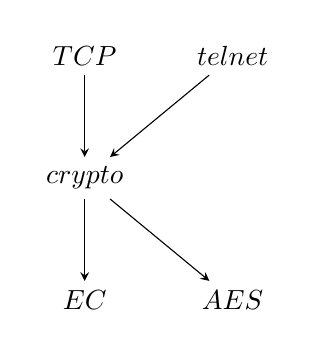
\begin{tikzpicture}
  \matrix (m) [matrix of math nodes,row sep=3em,column sep=2em,minimum width=2em]
  {
   TCP & telnet\\
   crypto \\
   EC & AES\\
   };
  \path[-stealth]

    (m-1-1) edge node [left] { } (m-2-1)
    (m-1-2) edge node [left] { } (m-2-1)
    
    (m-2-1) edge node [right] {} (m-3-1)

    (m-2-1) edge node [left] {} (m-3-2);   
\end{tikzpicture} 
\end{center}
De communicatie verloopt als volgt. Stel we verbinden als Client C met een server S. Als eerste stap zal de server alle andere gebruikers op de hoogte stellen dat er een nieuw iemand meeluistert, ook reageert de server met de eerste stap van het DH protocol op C. De Client stuurt zelf ook de eerste stap van het DH protocol op. Vervolgens berekenen zowel de Server S als de Client C het gedeelde geheim. Van dit geheim worden deelsleutels gemaakt die de up- en downstream van en naar de server beveiligen. Als C een bericht wil sturen aan de anderen die verbonden zijn met de server, versleutelt C zijn bericht met de upstream sleutels naar de server. Vervolgens verstuurt C dit bericht naar de server. De server ontvangt dit bericht en ontsleutelt deze met de upstream sleutel van C naar de server. Nu heeft de server het bericht dat C aan alle andere clients wilde sturen. Vervolgens genereert de server voor elke client $\tilde{C}$ een eigen versleuteling van het bericht met de downstream sleutels van $\tilde{C}$ naar de server. Vervolgens verstuurt de server dit bericht naar $\tilde{C}$. $\tilde{C}$ ontvangt dan dit bericht en kan met zijn downstream sleutel dit bericht ontsleutelen. 
\subsubsection{EC.py}
Dit bestand bevat alles wat nodig is om met de elliptische krommen te kunnen werken. De klasse FiniteFieldElem, die er is om te zorgen dat er in het eindige lichaam gewerkt kan worden in combinatie met de elliptische kromme, heeft de variabele $p$ om $\mathbb{F}_p$ te kunnen vormen voor $p$ priem.\\ De klasse Curve heeft twee variabelen, $a$ en $b$, zoals eerder om de kromme te defini\"{e}ren en $p$ om aan te geven op welk eindig lichaam (finite field) we werken.\\
De klasse Punt stelt een punt op een kromme voor, de variabelen x en y zijn FiniteFieldElem's, de klasse Eenheid is een subklasse van Punt en stelt het eenheidselement voor.
\subsubsection{AES\_good.py}
Dit bestand zorgt ervoor dat tekst versleuteld kan worden door middel van AES. Als begin hebben we een implementatie van AES van het internet afgeplukt die een blok van 16 bytes versleutelde met behulp van een 16 byte sleutel. Vervolgens hebben we deze code aangepast zodat hij een willekeurig lange stroom data kan versleuten, met behulp van codebookchaining. Deze module moet geinitialiseerd worden met een masterkey en een iv (initialisatie vector). De masterkey genereert de rondesleutels, en deze moet elke sessie willekeurig gekozen worden, of tot stand komen door een betrouwbaar key agreement protocol, en geheim blijven. De iv hoeft alleen willekeurig te zijn. Bij een gefixeerde iv, of niet willekeurig gekozen iv daalt het aantal berichten die veilig versleuteld kunnen worden zonder collisies.
\subsubsection{Crypto.py}
Dit bestand bevat de klasse LSEC, wat defini\"eert op welke kromme en eindig lichaam we werken en de klasse crypto.
De klasse crypto gebruikt zowel AES.py als EC.py, de laatste hiervan om een sleutel af te spreken, AES om de versleuteling van de berichten te doen. Na de versleuteling worden de berichten ondertekend met een HMAC gebaseerd op SHA256. Er is gekozen voor encrypt then sign omdat deze methode veel minder gevoelig is voor side channel aanvallen, en dezelfde theoretische veiligheid biedt. \\Verder wordt in Crypto.py gezorgd dat als er een gemeenschappelijke sleutel is afgesproken, er via herhaald hashen, via pbkdf2 (password-based key derivation function 2) hmac, veilige sleutels en iv's worden verzorgd voor de upstream en downstream van gegevens, de iv voor die streams en de sleutels om die streams te ondertekenen met behulp van HMAC.
\subsubsection{tcp.py}
tcp.py is de Pythonfile met daarin de server code. Deze houdt alle users bij met hun sleutels, en als er een bericht binnenkomt dan stuurt de server dit bericht door naar alle andere gebruikers van de server. De server gebruikt crypto.py om de berichten te versleutelen en met de clients sleutels af te spreken.
\subsubsection{telnet.py}
De Pythonfile telnet.py is de file voor de client en zorgt dat hij verbinding kan leggen met de server en kan communiceren. De client heeft in tegenstelling tot de server geen verbinding met alle gebruikers van de server, maar alleen met de server zelf. 
\newpage
\section{Aanvallen op de implementatie}
We bespreken in deze sectie enkele aanvalsmogelijkheden die een aanvaller hebben om het verkeer te onderscheppen. Ten eerste kan iedereen verbinding maken met de server waarop er gecommuniceerd wordt en het gesprek afluisteren. Maar als iemand verbinding maakt wordt dit bericht naar alle andere gebruikers gepushed en zijn alle gebruikers op de hoogte dat er iemand meeluistert. Er zijn ook andere methoden waarop de gebruikers niet op de hoogte hoeven te zijn dat er iemand meeluistert. Het protocol kan echter gemakkelijk worden aangepast zodat mensen zich moeten identificeren via een wachtwoord voordat ze mee mogen luisteren. Dit vergt een paar kleine aanpassingen voor de communicatie zelf. Echter wordt het problematisch om jezelf bij de server te registreren als ongeregistreerde berichten genegeerd worden. Hier zal een middenweg in gezocht moeten worden.
\subsection{Man in the middle}
Iemand zou zich kunnen voordoen als een betrouwbare server door al het verkeer af te luisteren. Vervolgens kan deze persoon dit verkeer doorsluizen naar de echte server en tegen de server doen alsof hij de client is. Omdat ip-pakketten vervalst kunnen worden, kan dit worden gedaan zonder dat de gebruikers er iets van merken. 
\subsection{Server omkopen}
Omdat al het verkeer via de server wordt geleid en de server over alle sleutels beschikt, kan een kwaadwillende server al het verkeer prijsgeven. 
\subsection{Side channel aanvallen}
Onze server is niet beveiligd tegen alle side channel aanvallen. Onze DH suite is lichtgevoelig voor timing-aanvallen en die zouden gebruikt kunnen worden om de interne staat van de klasse random te verraden. De klasse random is niet cryptografisch veilig en iemand kan daarmee gegevens over de geheime sleutel van de client bemachtigen. Deze geven dan de mogelijkheid om de gedeelde sleutel te bemachtigen want met de geheime sleutel en de publieke transactie kan alles worden afgeluisterd.
\\Na de Key-Exchange zijn er geen side channel-aanvalmogelijkheden bekend die van een afstand uit te voeren zijn. We gebruiken encrypt-then-sign omdat deze robuuster is tegen side channel aanvallen.

\subsection{Theoretische aanvallen}
Er bestaan ook aanvallen tegen AES en DH. Deze aanvallen zijn puur theoretisch op dit moment en zijn praktisch niet haalbaar. Als het discrete logaritme probleem wordt opgelost zou dit een flinke klap zijn voor de veiligheid van versleutelings algoritmen gebaseerd op Diffie-Hellman sleutel uitwisseling. Daarentegen zijn elliptische krommen resistanter dan andere varianten van het Diffie-Hellman protocol. Verder zou het kunnen dat AES gebroken wordt en er een ciphertext aanval komt. Dit is echter onwaarschijnlijk aangezien AES een goed onderzocht protocol is, gebaseerd op wiskundig goed onderbouwde methoden. Ten derde zou men een aanval tegen bijvoorbeeld SHA256 kunnen vinden, zodat de message authenticatie vervalst kan worden en mensen daarna side channel aanvallen tegen gewoon cbc AES gaan doen via adaptive chosen ciphertext, zoals de aanval die eerder besproken is. Deze aanval wordt bemoeilijkt in onze code, omdat de code die we geschreven hebben geen resultaat terug geeft over hoe lang het duurde om alles te ontsleutelen en of de ontsleuteling gelukt is. Dus via deze methode kun je ook geen delen van de data terugvinden.
\newpage
\section{Conclusie}
We hebben in dit project een applicatie geschreven waarbij men redelijk veilig kan communiceren over het internet. Als een user eenmaal veilig de verbinding tot stand heeft gebracht, kan men moeilijk het verkeer af luisteren. De optie om de servereigenaar om te kopen en de geheimen prijs te geven blijft echter altijd bestaan. Een manier om dit te voorkomen is de server en een van de clients op dezelfde computer te draaien en via andere communicatie af te spreken wie de server beheert.

\section{Taakverdeling}
Onze taakverdeling was als volgt: telnet.py, tcp.py, AES\_good.py zijn door Stefan aangepast van internetbronnen om te voldoen aan wat wij ermee wilden doen. Stefan heeft ook het grootste deel van crypto.py en FiniteField in EC.py geschreven. Roald heeft de code die nog over is geschreven en daarnaast geholpen met debuggen van de code. Dit verslag is geschreven door Roald waarbij Stefan geholpen heeft, het stuk over AES encryptie en aanvallen is geschreven door Stefan. 
\section{Looptijden van algoritmen}
Bijna al onze methodes zijn $O(1)$. Uitzonderingen daarop zijn bijvoorbeeld de methodes die de berichten verwerken, deze zijn lineair in de grootte van het bericht. De methode om punten te vermenigvuldigen met scalars wordt uitgevoerd in $O(\log(\text{scalar}))$, zo ook de machtsverheffing van FiniteFieldElem's $O(\log(\text{macht})$. Andere zijn... (Maak even af Stefan :P).
\section{Bugs}
Helaas is het ons niet gelukt de code compleet bug-vrij af te leveren. De volgende bugs zijn wij bekend mee: het programma werkt niet op Windows, reden hiervoor is dat de implementatie van hoe Python3 met sockets omgaat in Windows niet werkt. De pijltjestoetsen worden opgepakt als meerdere leestekens, deze zouden genegeerd moeten worden of de typcursor moeten verplaatsen. "Onverwachts verbinding verbreken" kan ervoor zorgen dat de Broken pipe-error wordt geraised, dit zou bijvoorbeeld deels opgelost kunnen worden door een codewoord te implementeren die je bij de server afmeldt. 

%\section{gebruikte bronnen}
\begin{thebibliography}{9}
\bibitem{client} http://www.binarytides.com/code-chat-application-server-client-sockets-python/\\
\bibitem{AES} https://github.com/bozhu/AES-Python\\
\bibitem{Field}Weisstein, Eric W. "Field Axioms." From MathWorld--A Wolfram Web Resource.\\ http://mathworld.wolfram.com/FieldAxioms.html \\
\bibitem{Vieta}Weisstein, Eric W. "Vieta's Formulas." From MathWorld--A Wolfram Web Resource. http://mathworld.wolfram.com/VietasFormulas.html\\
\bibitem{Rijndael}http://csrc.nist.gov/archive/aes/rijndael/Rijndael-ammended.pdf\\
\bibitem{jeremykun}http://jeremykun.com/2014/02/08/introducing-elliptic-curves/
\end{thebibliography}
Bronnen voor de code staan vermeld in de Python3 bestanden zelf.
\end{document}
